Os resultados obtidos abrangem várias etapas importantes do projeto, até o presente momento. Inicialmente, incluem a prototipagem das telas da aplicação móvel, que posteriormente será traduzida e compilada utilizando uma linguagem de programação adequada para ser implementada no Sistema em Node.js, destinado ao uso em desktop. Além disso, são apresentados os estudos realizados para o Business Model Canvas, bem como a modelagem do banco de dados, tanto no nível conceitual quanto lógico. Essa modelagem inclui os Diagramas de Classe e de Objetos, os quais estão segmentados pelos perfis do Professor e do Estudante, detalhando as correlações das entidades com seus atributos específicos.
\\

Adicionalmente, são elaboradas as estruturas sistêmicas na forma do Diagrama de Caso de Uso (DCU), os quais são diferenciados de acordo com os perfis do Professor e do Estudante. Estes diagramas destacam as permissões e acessos individuais de cada usuário no sistema. Por fim, é apresentado o Diagrama de Rede, ilustrando a maneira pela qual os usuários acessam e transmitem dados dentro da aplicação.
\\

Além das etapas mencionadas, são realizados cálculos para verificar a eficácia do algoritmo de ordenação implementado no sistema. Esses cálculos são cruciais para avaliar o desempenho e a eficiência do algoritmo em diferentes cenários.
\\

\begin{itemize}

\item \textbf{Business Model Canvas}
\\

\end{itemize}

O desenvolvimento de um modelo de negócios demanda uma atenção primordial na satisfação das necessidades e expectativas do cliente. Para viabilizar o Sistema de Trilha Pedagógica Gamificada, é essencial conduzir estudos e investir no âmbito da tecnologia educacional e das metodologias direcionadas ao desenvolvimento curricular, seja em formato digital, conectado ou offline. Além disso, é imperativo estabelecer parcerias estratégicas com redes de ensino, setor privado e empresas especializadas no desenvolvimento de ferramentas educacionais, as quais contribuirão para a concretização dos objetivos delineados no Business Model Canvas (\Cref{fig:imgBMC.jpg}).
\\

\begin{figure}[!h]
\centering
\caption{BUSINESS MODEL CANVAS - TPG System}%
\label{fig:imgBMC.jpg}
\includegraphics[scale=0.3]{Illustrations/imgBMC.jpg}
\SourceOrNote{Autoria Própria (2024)}
\end{figure}
\pagebreak

\begin{itemize}

\item \textbf{Prototipação do Sistema Mobile - Figma:}
\\

\end{itemize}

A (\Cref{fig:Tela1}) mostra a tela inicial do TPG System, acessada pelo dispositivo móvel. Este sistema permite que o usuário realize seu cadastro (\Cref{fig:Tela2}), caso seja a primeira vez que estiver acessando, ou faça login (\Cref{fig:Tela3}), escolhendo seu perfil de Professor ou Estudante para prosseguir.
\\

\begin{figure}[!h]
\centering
\caption{Tela de Apresentação do Sistema - TPG System}%
\label{fig:Tela1}
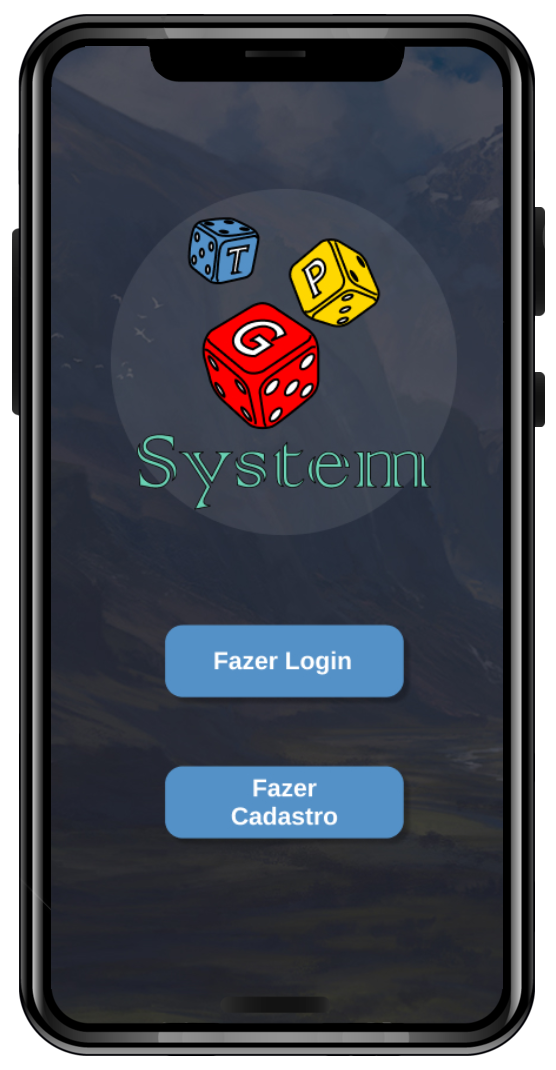
\includegraphics[scale=0.20]{Illustrations/Tela1.png}
\SourceOrNote{Autoria Própria (2024)}
\end{figure}

\begin{figure}[!h]
\centering
\caption{Tela de Cadastro - TPG System}%
\label{fig:Tela2}
\includegraphics[scale=0.20]{Illustrations/Tela2.png}
\SourceOrNote{Autoria Própria (2024)}
\end{figure}

\begin{figure}[!h]
\centering
\caption{Tela de Login - TPG System}%
\label{fig:Tela3}
\includegraphics[scale=0.20]{Illustrations/Tela3.png}
\SourceOrNote{Autoria Própria (2024)}
\end{figure}
\\

No perfil de Professor, é liberado o acesso para a realização do “Cadastro da Aventura” (\Cref{fig:Tela4}), que oferece as seguintes opções de menu (\Cref{fig:Tela5}):
\\
\pagebreak

\begin{figure}[!h]
\centering
\caption{Perfil do Professor - Realização de Cadastro - TPG System}%
\label{fig:Tela4}
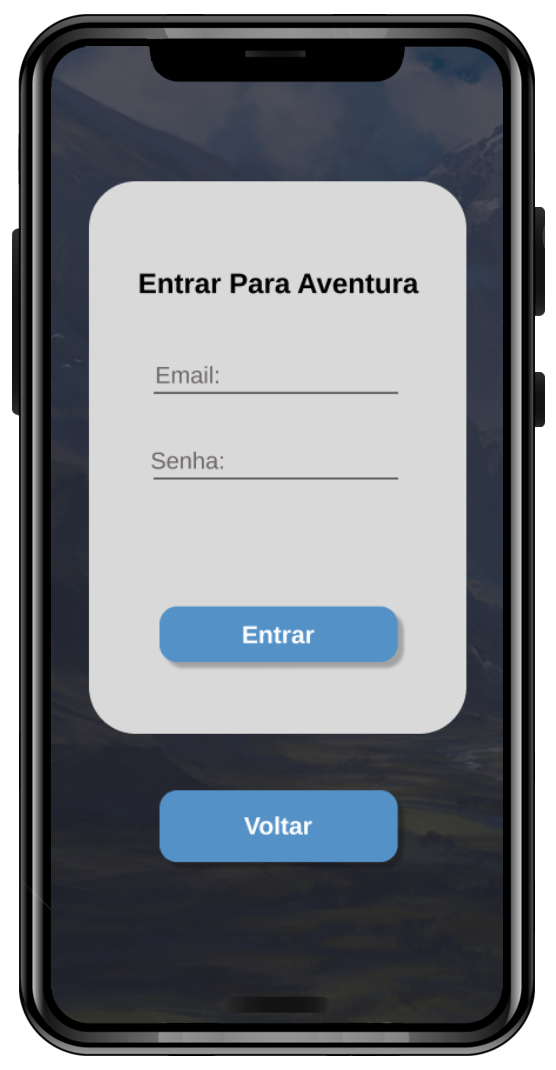
\includegraphics[scale=0.20]{Illustrations/Tela4.png}
\SourceOrNote{Autoria Própria (2024)}
\end{figure}

\begin{figure}[!h]
\centering
\caption{Perfil do Professor - Menu de Consultas e Opções - TPG System}%
\label{fig:Tela5}
\includegraphics[scale=0.20]{Illustrations/Tela5.png}
\SourceOrNote{Autoria Própria (2024)}
\end{figure}

“Iniciar”, onde o professor pode acompanhar o desenvolvimento dos usuários com o sistema, que reconhece as interações do usuário com os desafios, funcionando como um teste prático. Isso permite que o professor ajuste manualmente os níveis de dificuldade e as habilidades relacionadas;
\\

“Opções”, que abre uma nova tela (\Cref{fig:Tela6}), permitindo a consulta dos relatórios sistêmicos via desenvolvimento dos estudantes, na opção “Verificar Estudante”, disponível após a realização dos cadastros sistêmicos das turmas lecionadas, ou a criação de uma Nova Turma (\Cref{fig:Tela7});
\\

\begin{figure}[!h]
\centering
\caption{Perfil do Professor - Opções de Consulta de Relatórios ou Cadastro de Turmas - TPG System}%
\label{fig:Tela6}
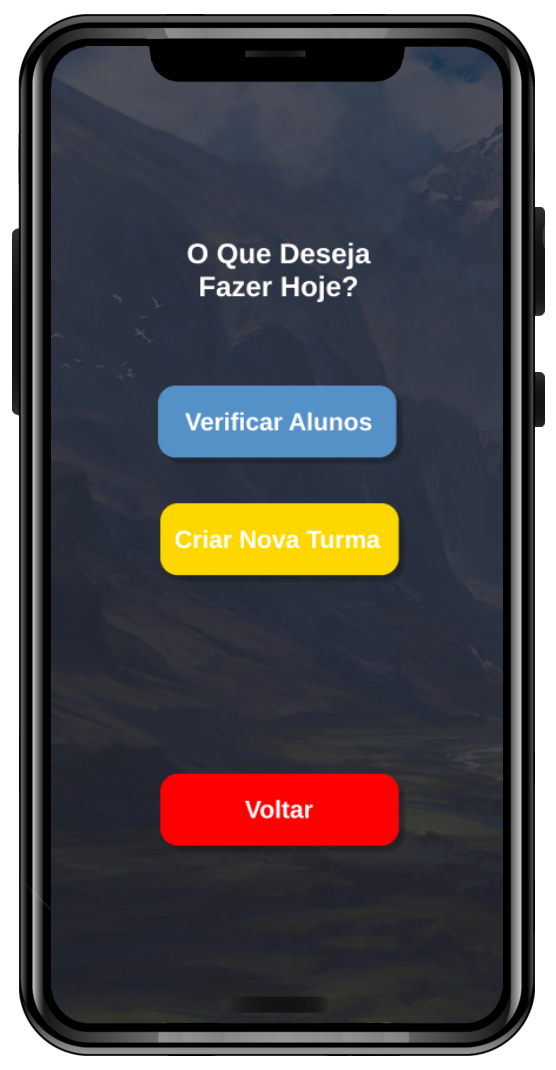
\includegraphics[scale=0.20]{Illustrations/Tela6.png}
\SourceOrNote{Autoria Própria (2024)}
\end{figure}

\begin{figure}[!h]
\centering
\caption{Perfil do Professor - Cadastro da Turma no sistema - TPG System}%
\label{fig:Tela7}
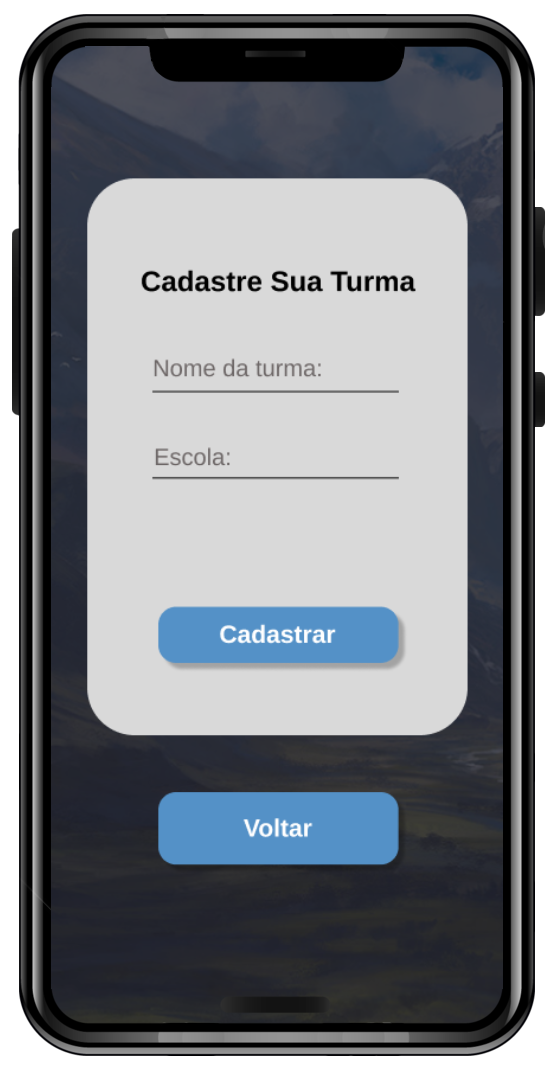
\includegraphics[scale=0.20]{Illustrations/Tela7.png}
\SourceOrNote{Autoria Própria (2024)}
\end{figure}

“Sair”, que realiza o logout do sistema.
\\
\pagebreak

No perfil de Estudante, é necessário realizar o “Cadastro de Aventureiro” (\Cref{fig:Tela8}) para liberar o acesso à criação de personagens (atualmente, o sistema oferece personagens prontos para uso e familiarização). Após o cadastro, o estudante pode explorar o sistema (\Cref{fig:Tela9}) e, ao logar-se, é direcionado para uma nova tela (\Cref{fig:Tela10}) com os seguintes menus:
\\

\begin{figure}[!h]
\centering
\caption{Perfil do Estudante - Cadastro de Aventureiro - TPG System}%
\label{fig:Tela8}
\includegraphics[scale=0.20]{Illustrations/Tela8.png}
\SourceOrNote{Autoria Própria (2024)}
\end{figure}

\begin{figure}[!h]
\centering
\caption{Perfil do Estudante - Acesso ao Sistema Pedagógico Gamificado - TPG System}%
\label{fig:Tela9}
\includegraphics[scale=0.20]{Illustrations/Tela9.png}
\SourceOrNote{Autoria Própria (2024)}
\end{figure}

\begin{figure}[!h]
\centering
\caption{Perfil do Estudante - Menus e Opções - TPG System}%
\label{fig:Tela10}
\includegraphics[scale=0.20]{Illustrations/Tela10.png}
\SourceOrNote{Autoria Própria (2024)}
\end{figure}

“Iniciar”, onde o estudante inicia a Trilha Pedagógica Gamificada, sendo direcionado ao ponto de partida no mapa relacionado ao personagem escolhido;
\\

“Opções”, onde o estudante pode verificar sua evolução no jogo, as conquistas obtidas e as derrotas nos desafios, apresentados em um relatório personalizado;
\\

“Sair”, que realiza o logout do sistema.
\\

Na tela “Qual Tema da sua Aventura?” (\Cref{fig:Tela11}), o estudante pode escolher trilhas específicas de acordo com seus interesses ou necessidades de desenvolvimento de habilidades e competências. Após selecionar o componente desejado, aparece um sub-menu com as aventuras disponíveis (\Cref{fig:Tela12}).
\\

\begin{figure}[!h]
\centering
\caption{Perfil do Estudante - Escolha de Temas (Componentes) - TPG System}%
\label{fig:Tela11}
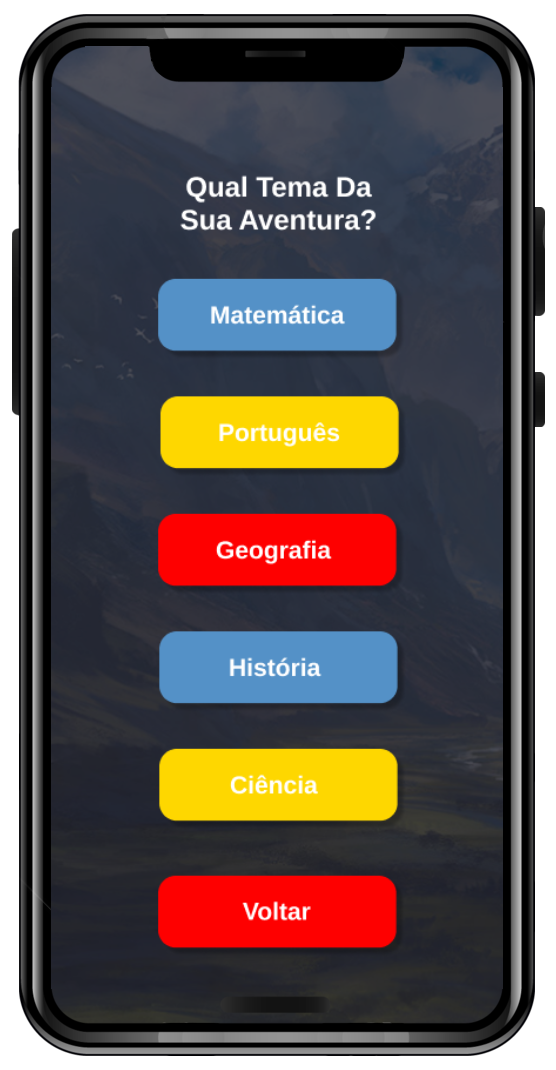
\includegraphics[scale=0.20]{Illustrations/Tela11.png}
\SourceOrNote{Autoria Própria (2024)}
\end{figure}

\begin{figure}[!h]
\centering
\caption{Perfil do Estudante - Escolha da Aventura dentro do Tema - TPG System}%
\label{fig:Tela12}
\includegraphics[scale=0.20]{Illustrations/Tela12.png}
\SourceOrNote{Autoria Própria (2024)}
\end{figure}

Ao iniciar o jogo, o estudante vê um mapa (\Cref{fig:Tela13}) com pontos de interesse que direcionam para desafios intelectuais ou de combate. Neste menu (\Cref{fig:Tela14}), o estudante pode consultar os dados de seu Personagem (\Cref{fig:Tela15}), bem como seu Inventário e as Informações de sua Conta, além de ter a opção de sair do sistema.
\\

\begin{figure}[!h]
\centering
\caption{Perfil do Estudante - Mapa da Aventura - TPG System}%
\label{fig:Tela13}
\includegraphics[scale=0.20]{Illustrations/Tela13.png}
\SourceOrNote{Autoria Própria (2024)}
\end{figure}

\begin{figure}[!h]
\centering
\caption{Perfil do Estudante - Menu - TPG System}%
\label{fig:Tela14}
\includegraphics[scale=0.20]{Illustrations/Tela14.png}
\SourceOrNote{Autoria Própria (2024)}
\end{figure}

\begin{figure}[!h]
\centering
\caption{Perfil do Estudante - Status do Personagem - TPG System}%
\label{fig:Tela15}
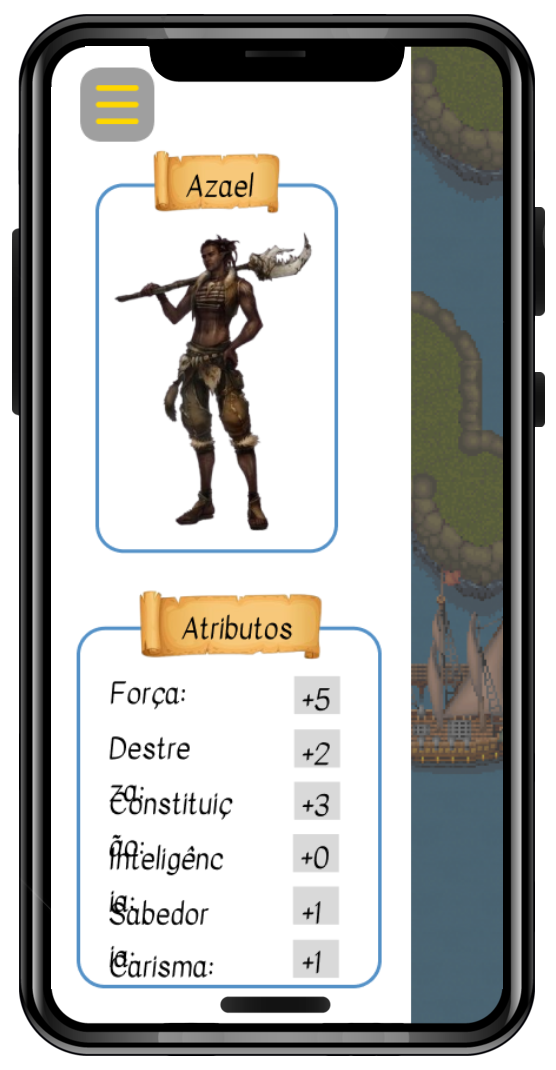
\includegraphics[scale=0.20]{Illustrations/Tela15.png}
\SourceOrNote{Autoria Própria (2024)}
\end{figure}
\\
\pagebreak
Está sendo estudada a possibilidade de que, ao sair, as informações de evolução não sejam perdidas, permitindo que, ao relogar no sistema, o estudante continue de onde parou. Este recurso possibilita uma continuidade na aprendizagem de forma dinâmica, sem a necessidade de reiniciar a etapa do zero.
\\
\pagebreak

\begin{itemize}

\item \textbf{Modelagem Banco de Dados - Conceitual e Lógico:}
\\

\end{itemize}

Na Modelagem Conceitual (\Cref{fcht:imgdgMC.jpg}), a ênfase foi dada à representação das associações entre as entidades, destacando seus atributos e, principalmente, os acessos através de chaves estrangeiras. Essa abordagem tem o objetivo de orientar a equipe de desenvolvimento na estruturação do sistema de forma a facilitar atualizações e modificações, permitindo a implementação rápida e precisa de novas funcionalidades. Esse estudo é solidificado por meio do diagrama da Modelagem Lógica (\Cref{fcht:imgdgML.jpg}), o qual representa de maneira mais concreta e detalhada as estruturas de dados e os relacionamentos definidos na etapa conceitual.
\\

\begin{flowchart}[!h]
\centering
\caption{Diagrama de Modelagem Conceitual - TPG System}%
\label{fcht:imgdgMC.jpg}
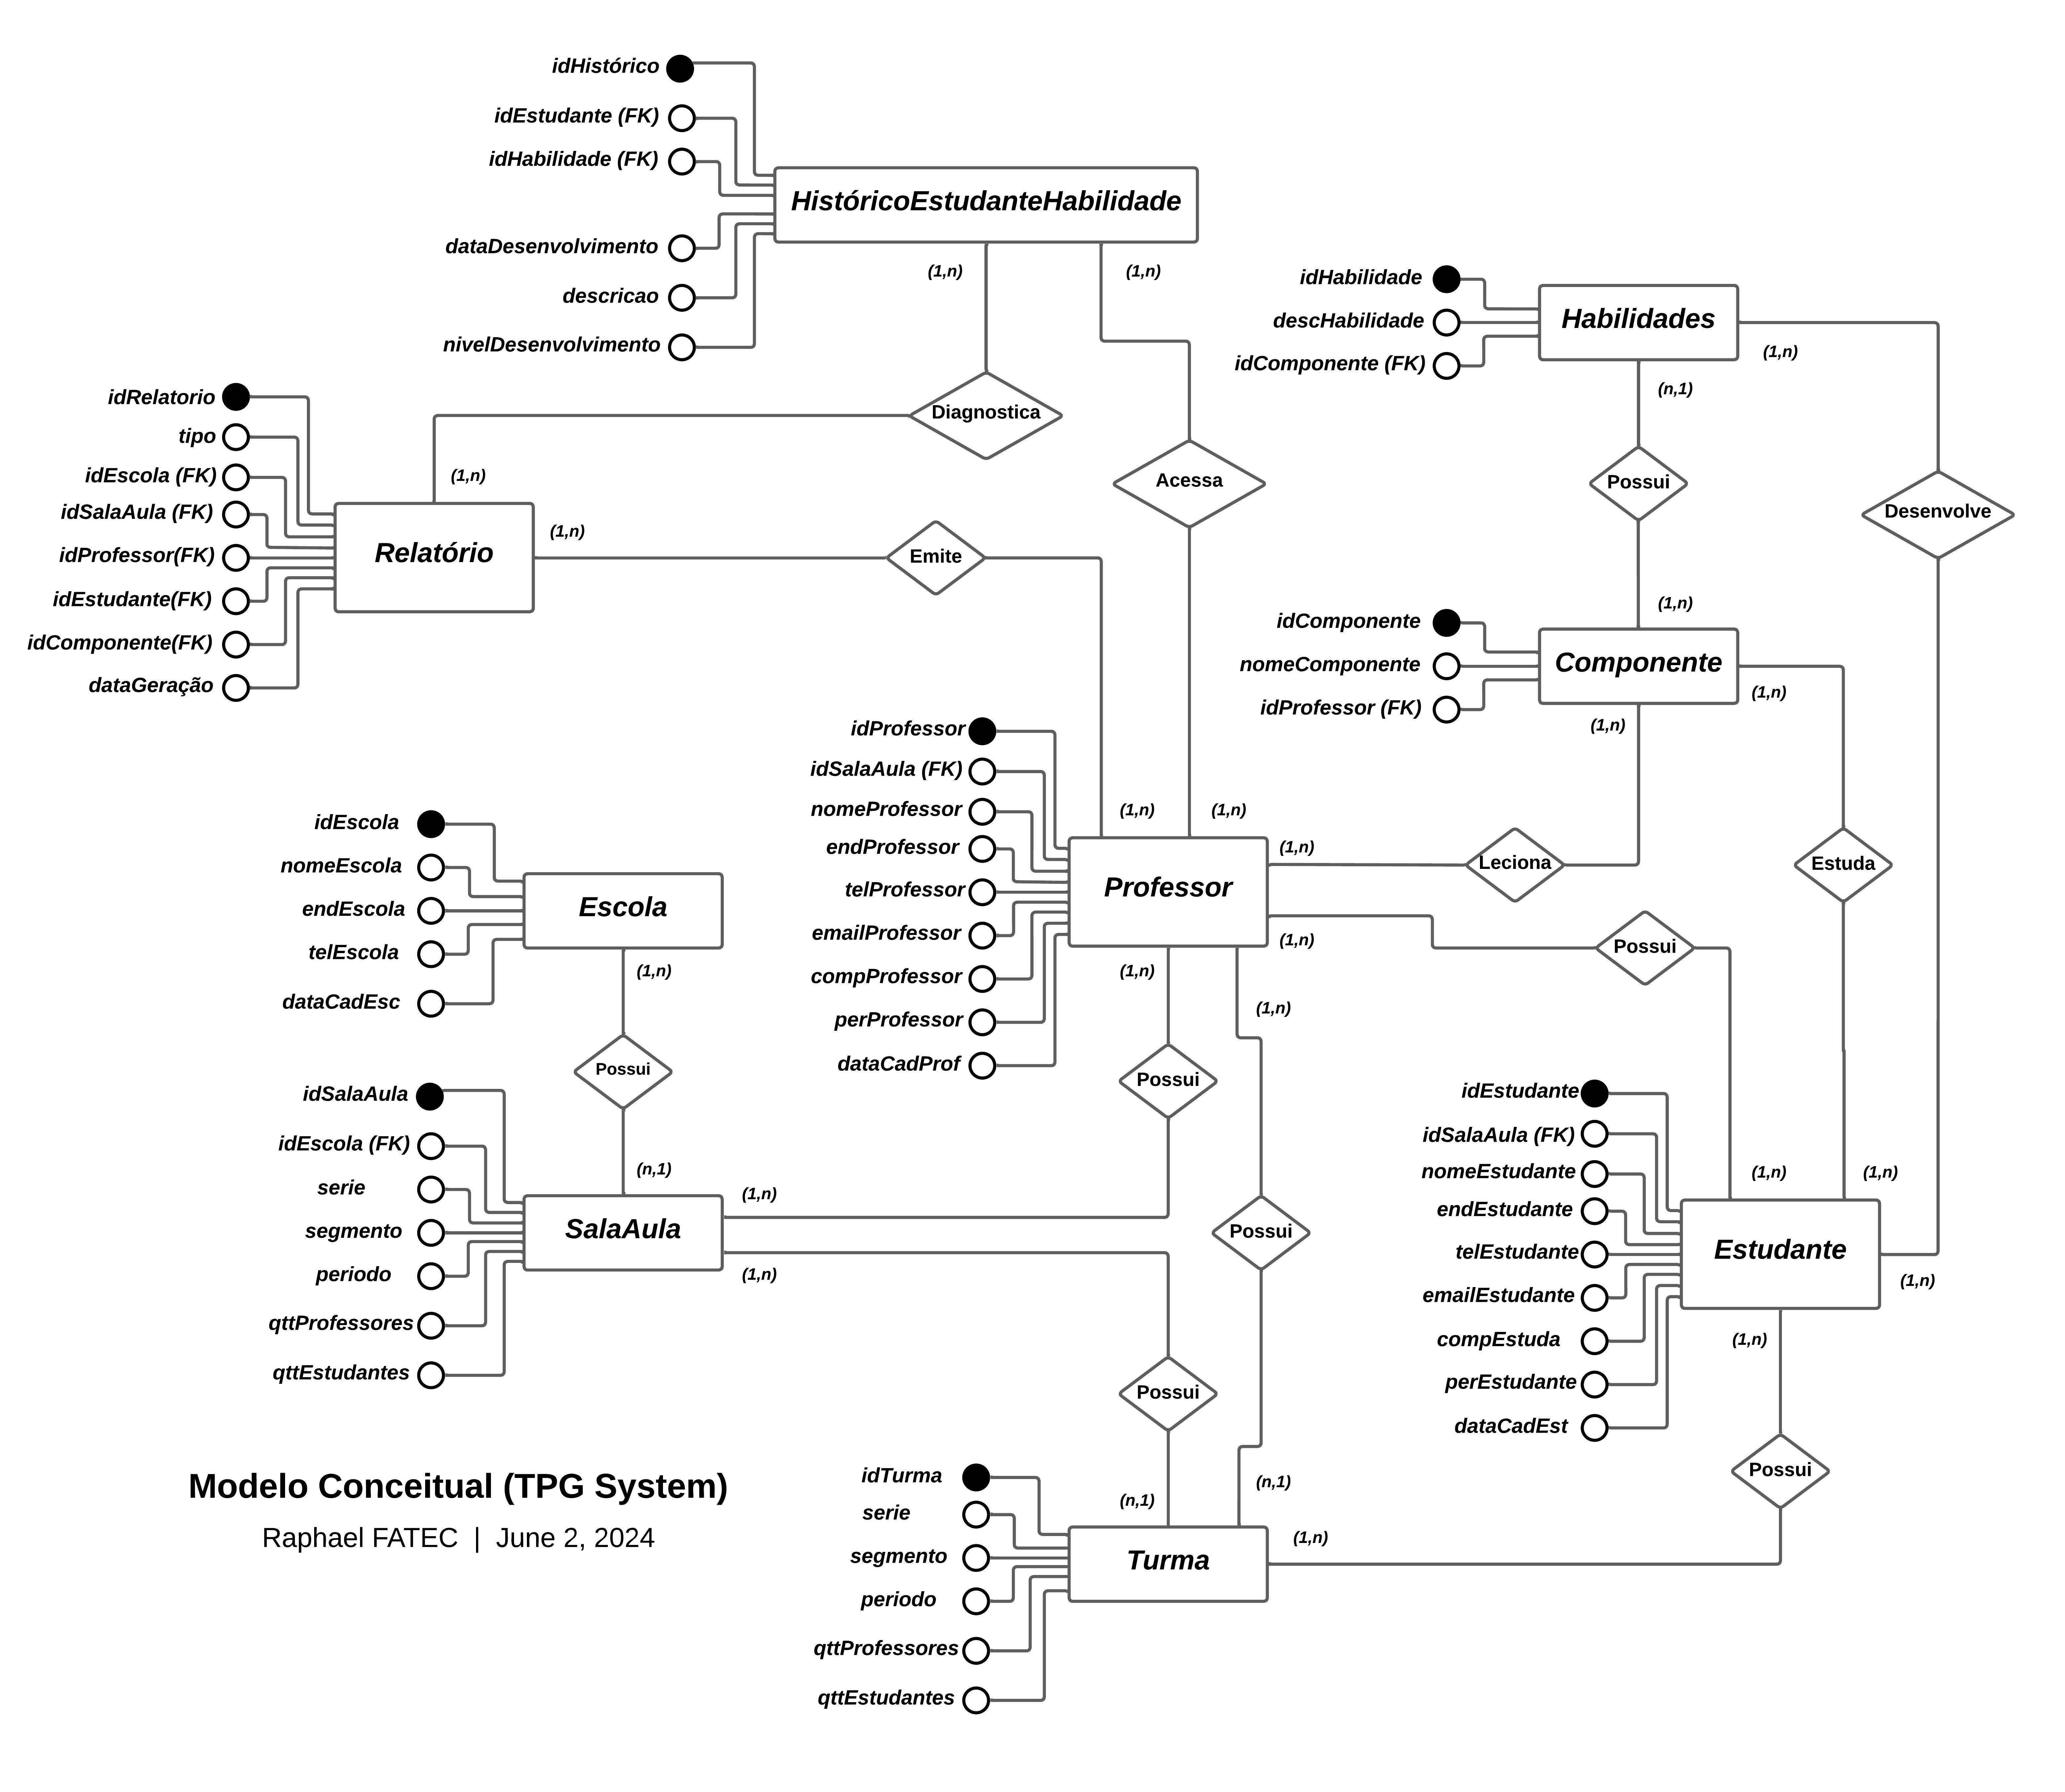
\includegraphics[scale=0.34]{Illustrations/imgdgMC.jpg}
\SourceOrNote{Autoria Própria (2024)}
\end{flowchart}
\\
\pagebreak

\begin{flowchart}[!h]
\centering
\caption{Diagrama de Modelagem Lógica - TPG System}%
\label{fcht:imgdgML.jpg}
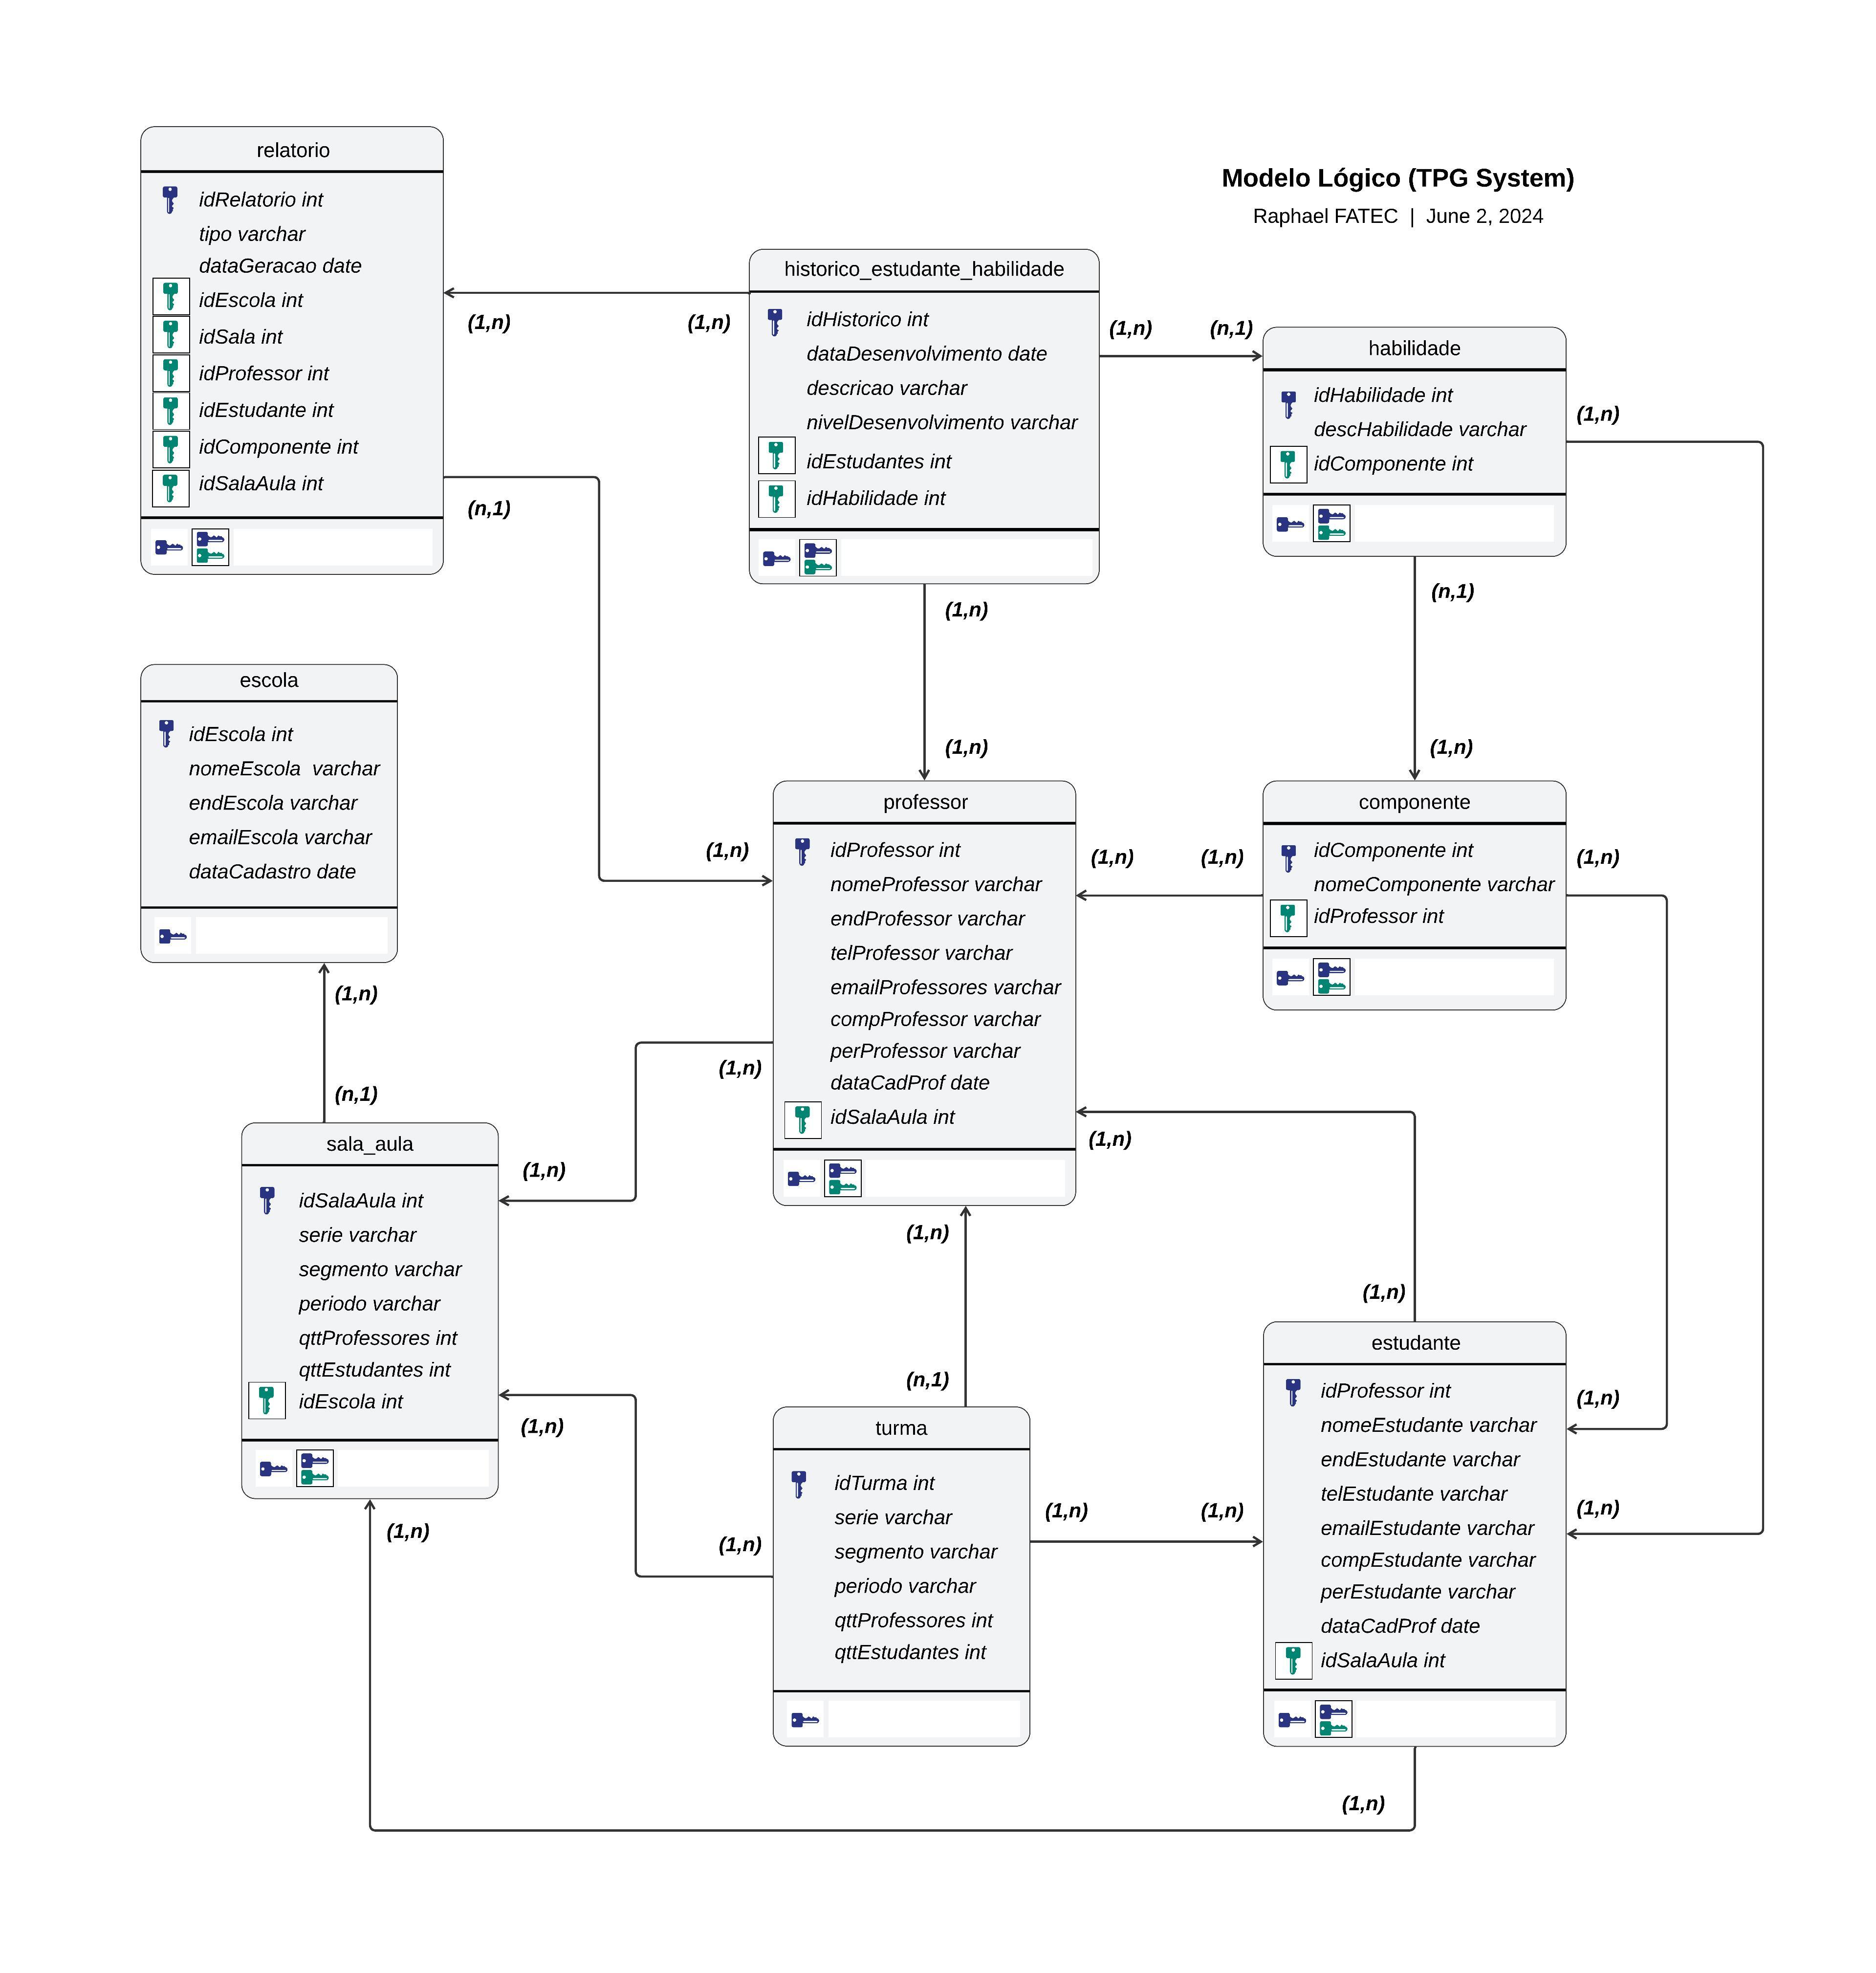
\includegraphics[scale=0.55]{Illustrations/imgdgML.jpg}
\SourceOrNote{Autoria Própria (2024)}
\end{flowchart}

\begin{itemize}

\item \textbf{Diagramas de Classe e Objeto:}
\\

\end{itemize}

No Diagrama de Classes do TPG System (\Cref{fcht:imgdgC.jpg}), podem-se observar diversas classes e seus relacionamentos, detalhando a estrutura de um sistema educacional com componentes curriculares, professores, alunos e desafios.
\\

\begin{flowchart}[!h]
\centering
\caption{Diagrama de Classe - TPG System}%
\label{fcht:imgdgC.jpg}
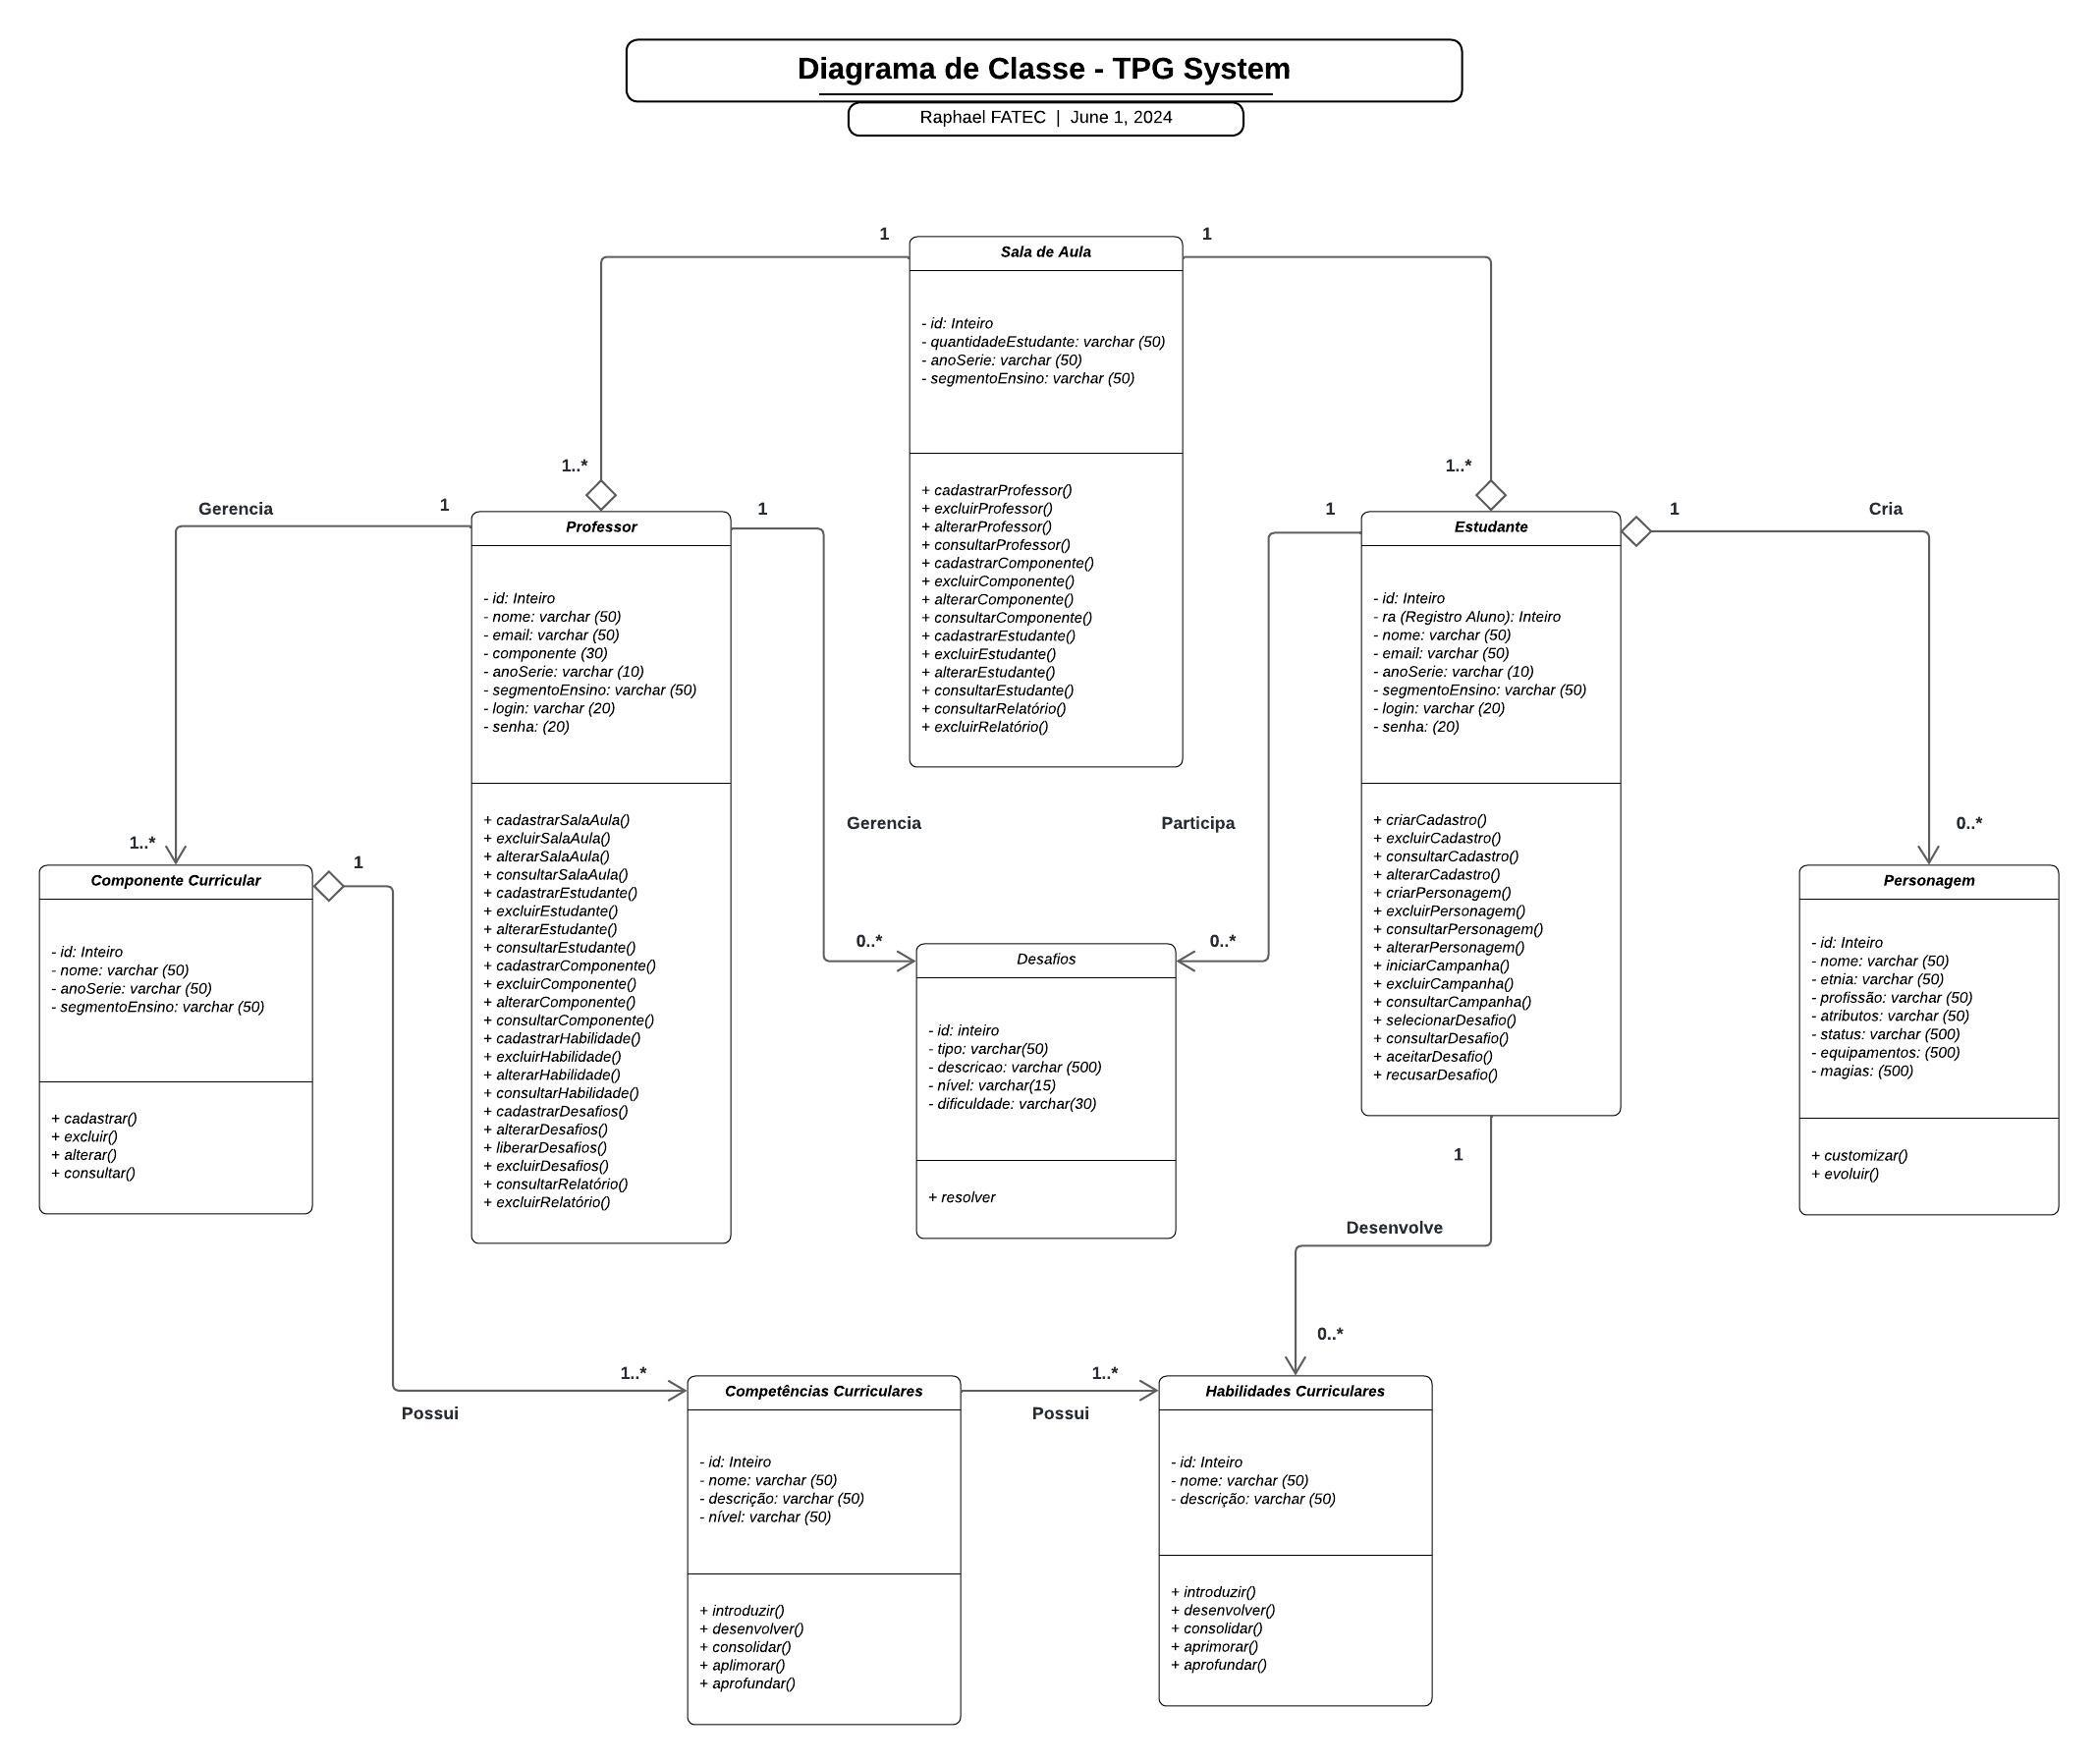
\includegraphics[scale=0.47]{Illustrations/imgdgC.jpg}
\SourceOrNote{Autoria Própria (2024)}
\end{flowchart}

Esse diagrama fornece uma visão abrangente da estrutura e dos relacionamentos essenciais para o funcionamento do sistema. Ao detalhar as classes, seus atributos e métodos, além das interações entre elas, o diagrama facilita a compreensão e a comunicação entre os desenvolvedores e outras partes interessadas, servindo como uma ferramenta de planejamento fundamental para a arquitetura do software.
\\

Nos Diagramas de Objetos, é apresentado o percurso do Professor (\Cref{fcht:imgdgObP.jpg}), detalhando o processo de cadastro e acesso sistêmico, bem como a importância de ter acesso aos recursos específicos do sistema. Isso permite que as informações necessárias possam ser incluídas, alteradas e consultadas de forma dinâmica e ordenada.
\\

\begin{flowchart}[!h]
\centering
\caption{Diagrama de Objeto (Professor) - TPG System}%
\label{fcht:imgdgObP.jpg}
\includegraphics[scale=0.50]{Illustrations/imgdgObP.jpeg}
\SourceOrNote{Autoria Própria (2024)}
\end{flowchart}

Quanto ao percurso do Estudante (\Cref{fcht:imgdgObE.jpg}), embora seja um caminho menos complexo no quesito de alimentação do sistema, pois ele já estará interagindo com as informações previamente inseridas pelo professor, exige um cuidado significativo para armazenar os dados de retorno. Isso é fundamental para subsidiar o sistema, permitindo a consulta, ordenação e geração de relatórios para o professor.
\\

\begin{flowchart}[!h]
\centering
\caption{Diagrama de Objeto (Estudante) - TPG System}%
\label{fcht:imgdgObE.jpg}
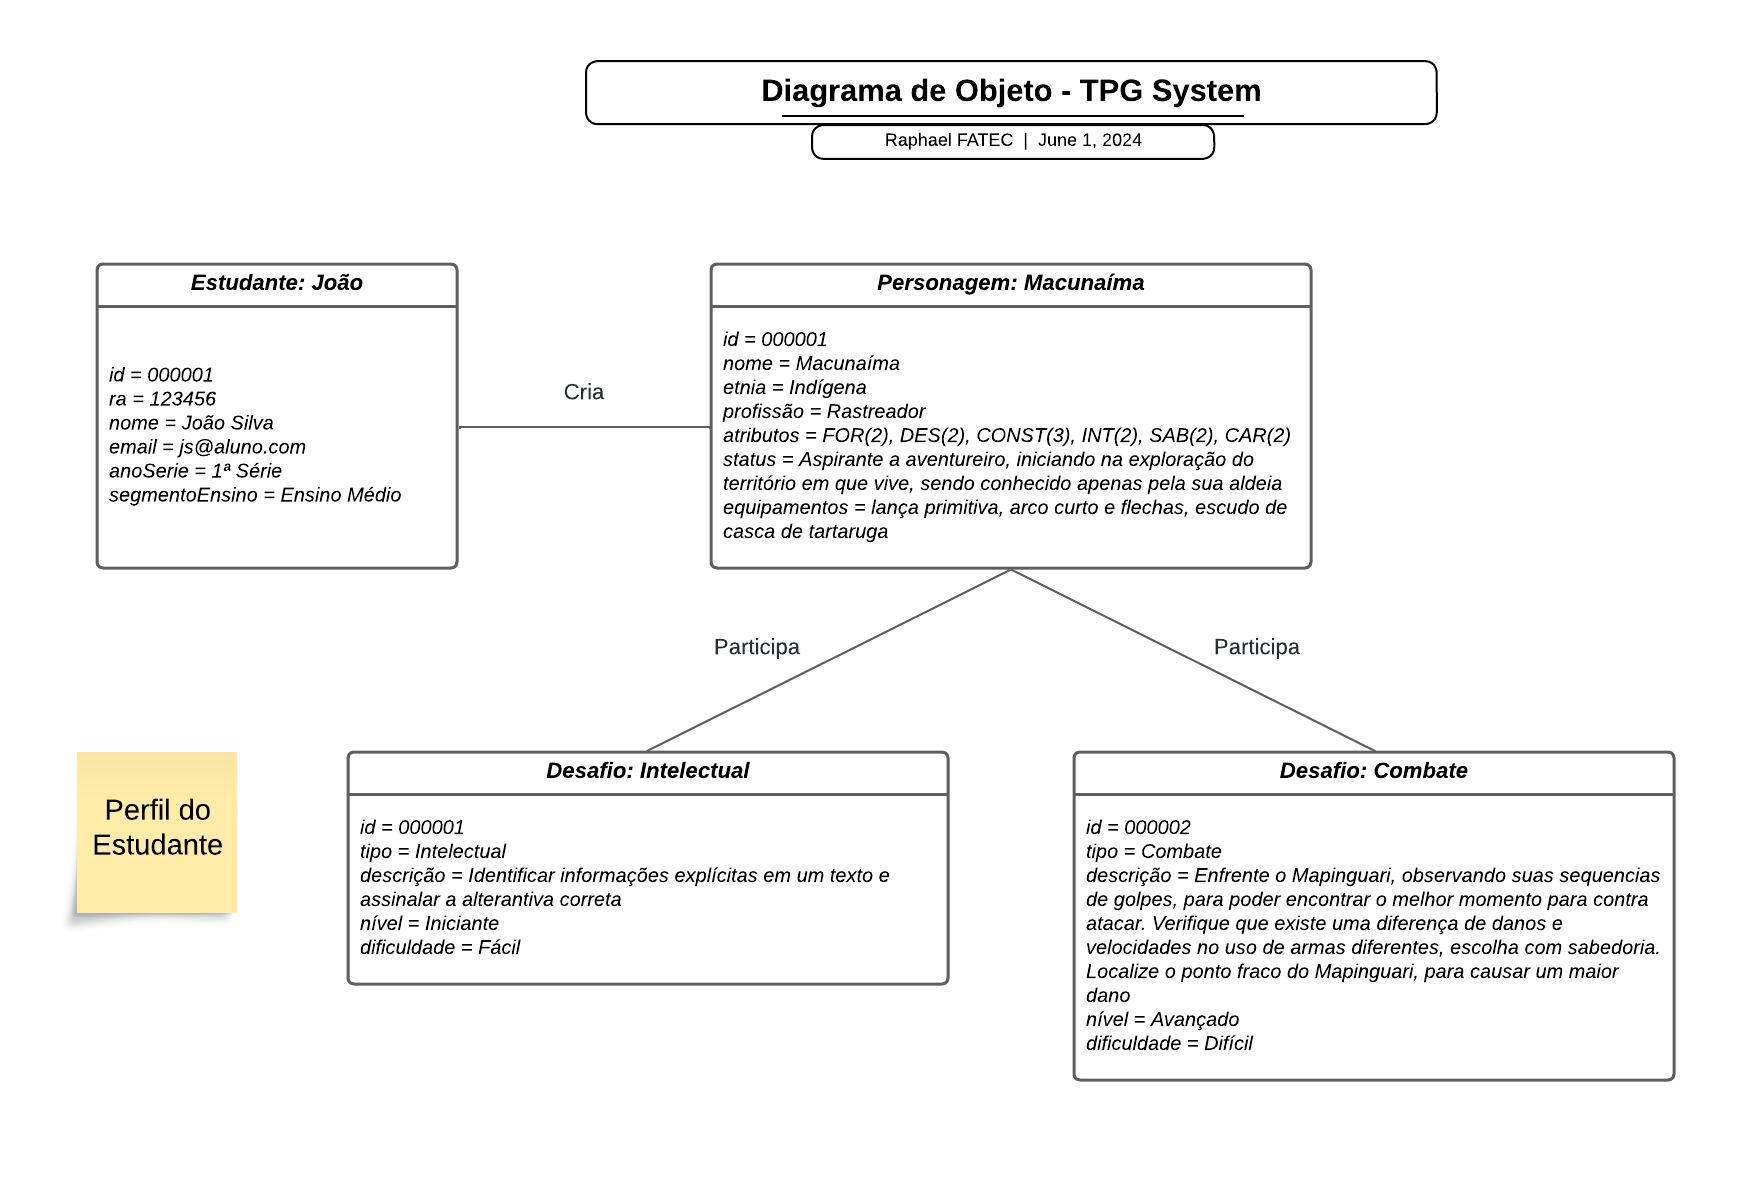
\includegraphics[scale=0.40]{Illustrations/imgdgObE.jpg}
\SourceOrNote{Autoria Própria (2024)}
\end{flowchart}

Esses diagramas fornecem exemplos concretos de como as classes e suas relações se manifestam em instâncias específicas dentro do sistema TPG. Eles ajudam a visualizar a estrutura do sistema educacional, mostrando como estudantes, professores, personagens e desafios interagem de maneira prática, facilitando o planejamento e desenvolvimento do software educacional
\\

\begin{itemize}

\item \textbf{Caso de Uso:}
\\

\end{itemize}


O processo de verificação e permissões no sistema resultou na estruturação do Caso de Uso em dois fluxogramas: o primeiro apresenta o Perfil do Professor (\Cref{fcht:imgdgCuP.jpg}), no qual é essencial o cadastro da Sala de Aula (representado em azul), ao qual o professor está vinculado, para a liberação do cadastro e acesso dos estudantes (representados em verde). Além disso, são fornecidas informações pertinentes sobre os Componentes que o professor leciona (representados em lilás), bem como a possibilidade de gerar os Relatórios Pedagógicos e acompanhar a evolução e/ou defasagem dos estudantes (representados em amarelo). É importante ressaltar que este fluxo deve ocorrer antes do cadastro pelos estudantes no sistema, visando facilitar a vinculação e cruzamento das informações.
\\

\begin{flowchart}[!h]
\centering
\caption{Diagrama de Caso de Uso - Perfil Professor - TPG System}%
\label{fcht:imgdgCuP.jpg}
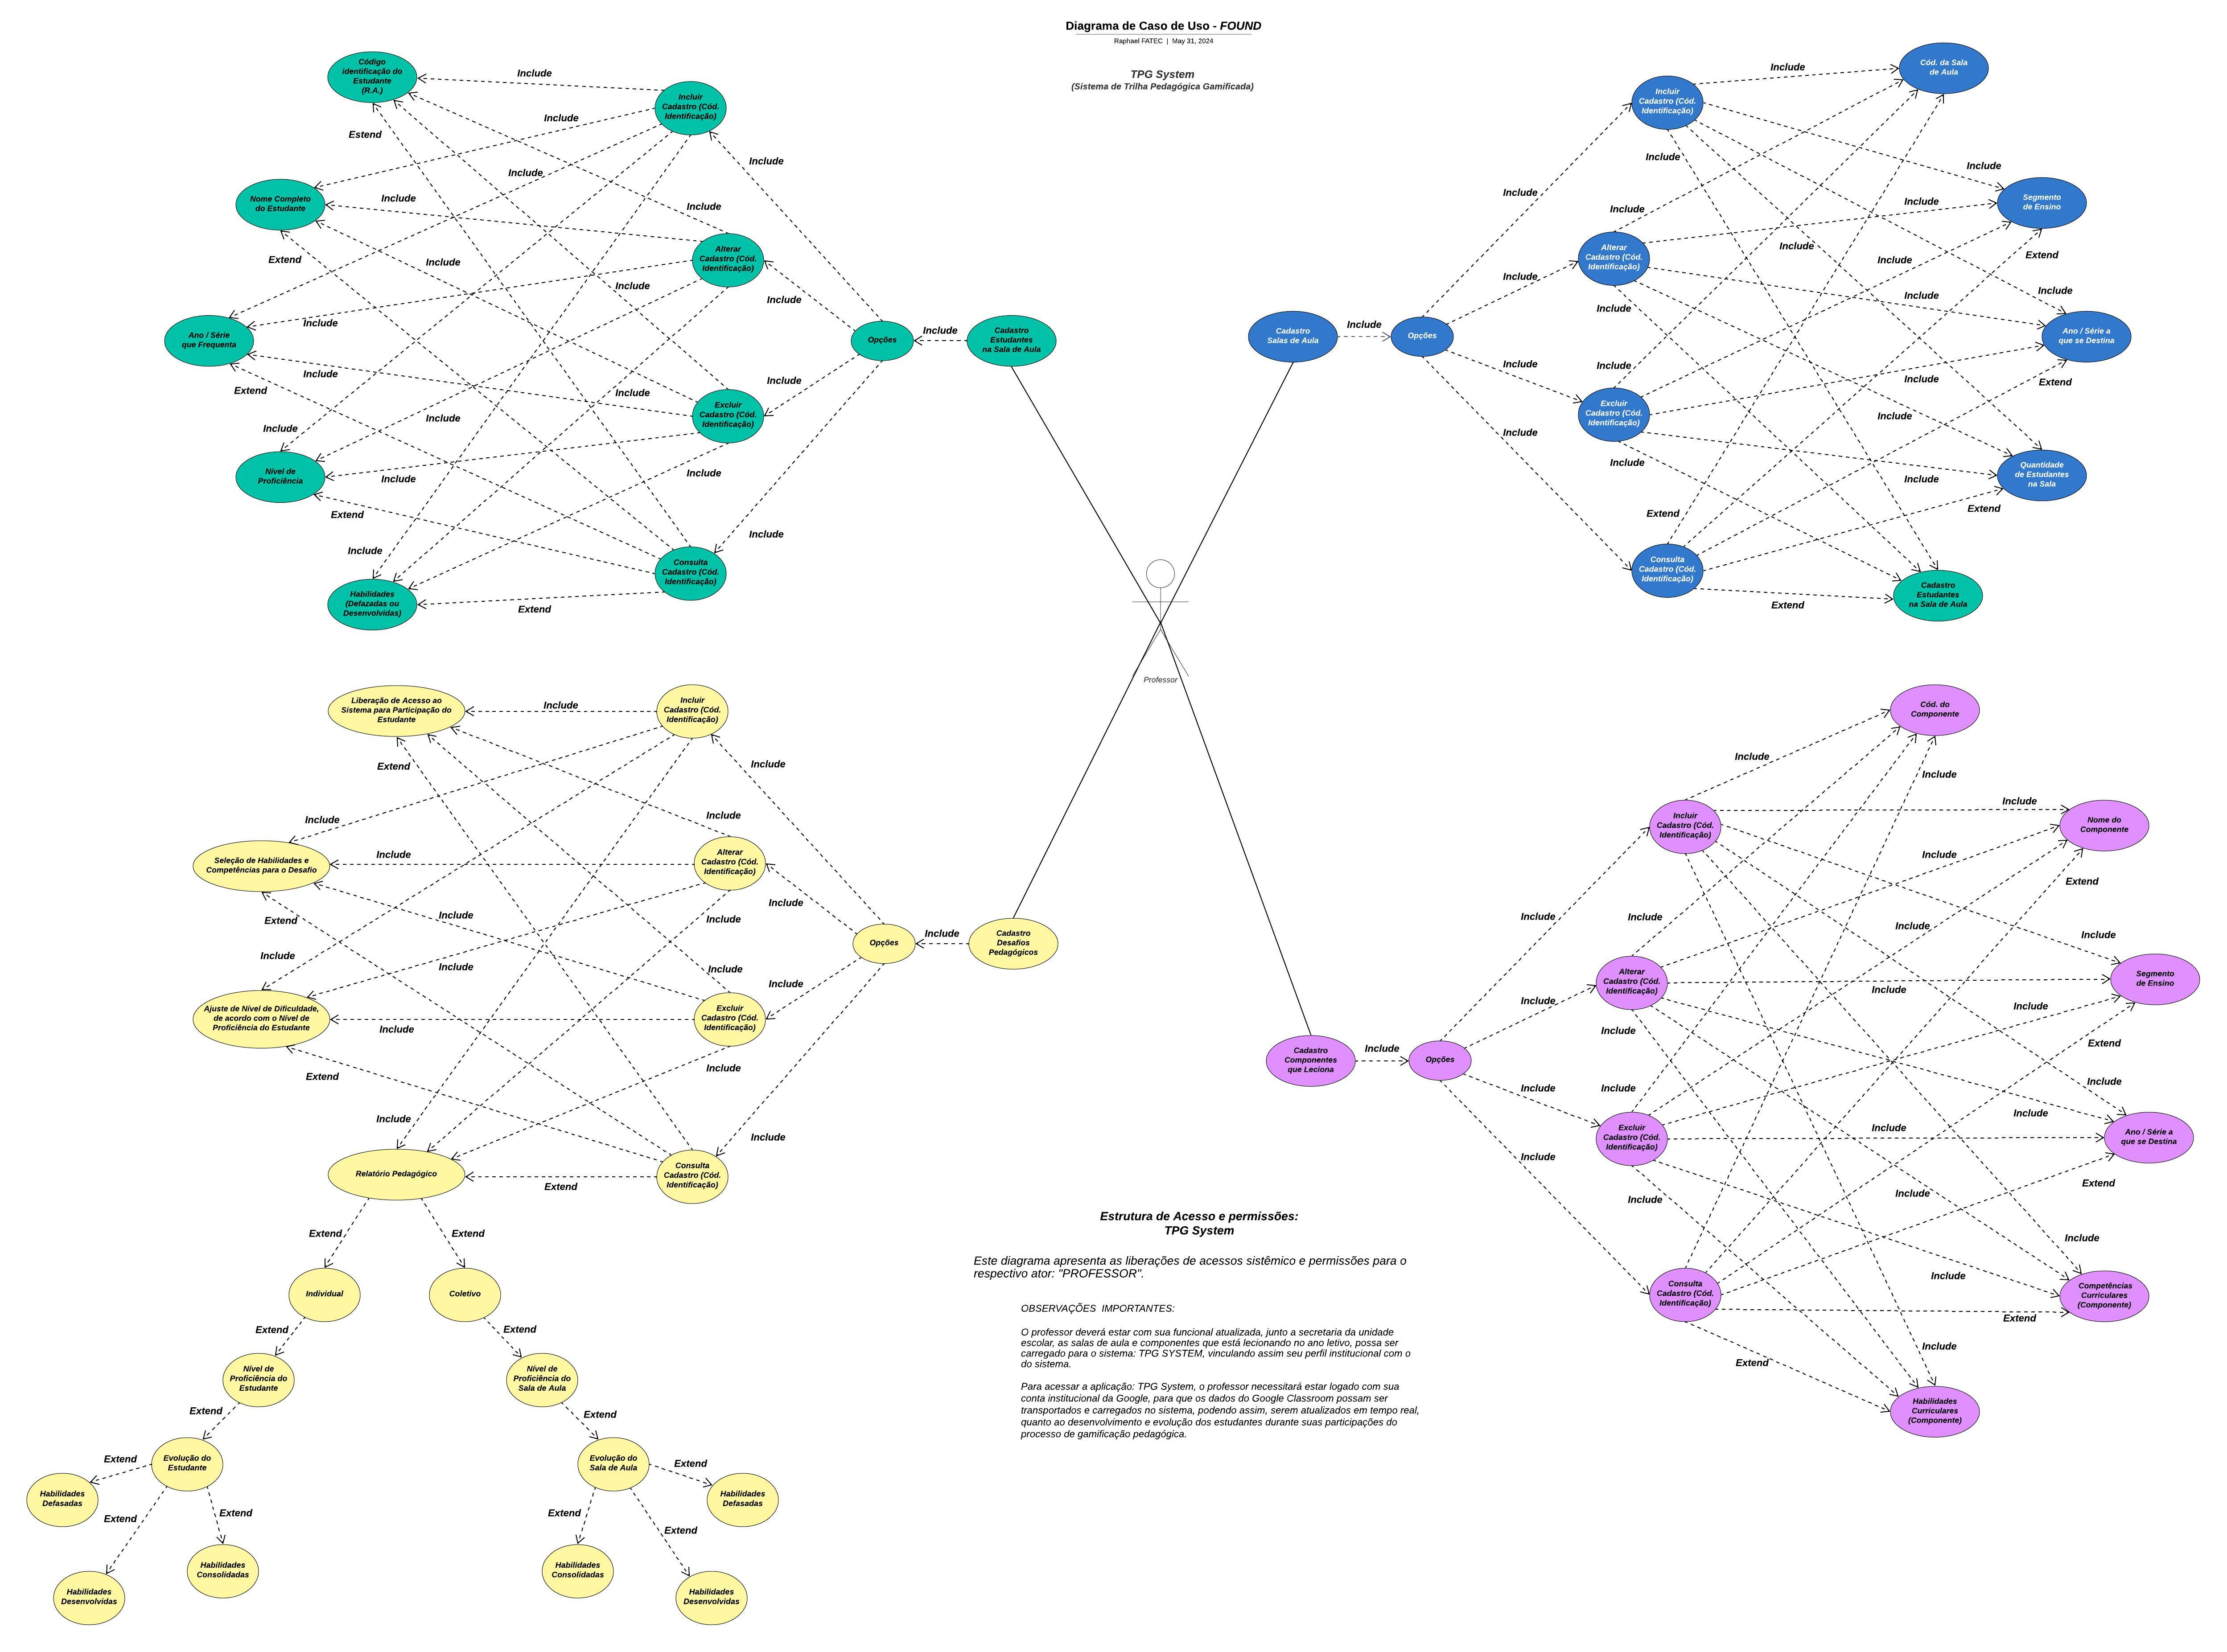
\includegraphics[scale=0.23]{Illustrations/imgdgCuP.jpg}
\SourceOrNote{Autoria Própria (2024)}
\end{flowchart}

Pelo Perfil do Estudante (\Cref{fcht:imgdgCuE.jpg}), nota-se que ele possui acesso interno ao sistema, podendo realizar a Criação de Seu Personagem (representado em azul claro) e iniciar propriamente o processo de participação efetiva no Sistema Pedagógico Gamificado, interagindo diretamente com a interface do sistema.
\\

\begin{flowchart}[!h]
\centering
\caption{Diagrama de Caso de Uso - Perfil Estudante - TPG System}%
\label{fcht:imgdgCuE.jpg}
\includegraphics[scale=0.33]{Illustrations/imgdgCuE.jpg}
\SourceOrNote{Autoria Própria (2024)}
\end{flowchart}

Dessa forma, pode-se inferir que o Professor atua mais como observador e mediador do processo, enquanto o verdadeiro protagonista é o Estudante. Entretanto, é importante ressaltar que os desafios e os níveis de dificuldade são estruturados pelo próprio sistema, com base nas informações fornecidas previamente pelo professor referentes às habilidades e competências do Componente Curricular. Isso possibilita que tais desafios sejam ofertados aos estudantes de forma adequada.
\\

Além disso, com base nas respostas dadas pelos estudantes, o sistema consegue estruturar os relatórios necessários para que o professor melhore suas estratégias pedagógicas e metodologias na sala de aula. Esses relatórios fornecem insights valiosos sobre o desempenho individual e coletivo dos alunos, permitindo ao professor ajustar suas abordagens de ensino de acordo com as necessidades identificadas.
\\

\begin{itemize}

\item \textbf{Diagrama de Rede:}
\\

\end{itemize}

O Diagrama de Rede (\Cref{fcht:dgR.jpg}), representa graficamente a estrutura, as atividades, dependências e o fluxo de trabalho do projeto. Esta ferramenta é fundamental no gerenciamento de projetos e oferece os seguintes benefícios:
\\

\begin{flowchart}[!h]
\centering
\caption{Diagrama de Rede - TPG System}%
\label{fcht:dgR.jpg}
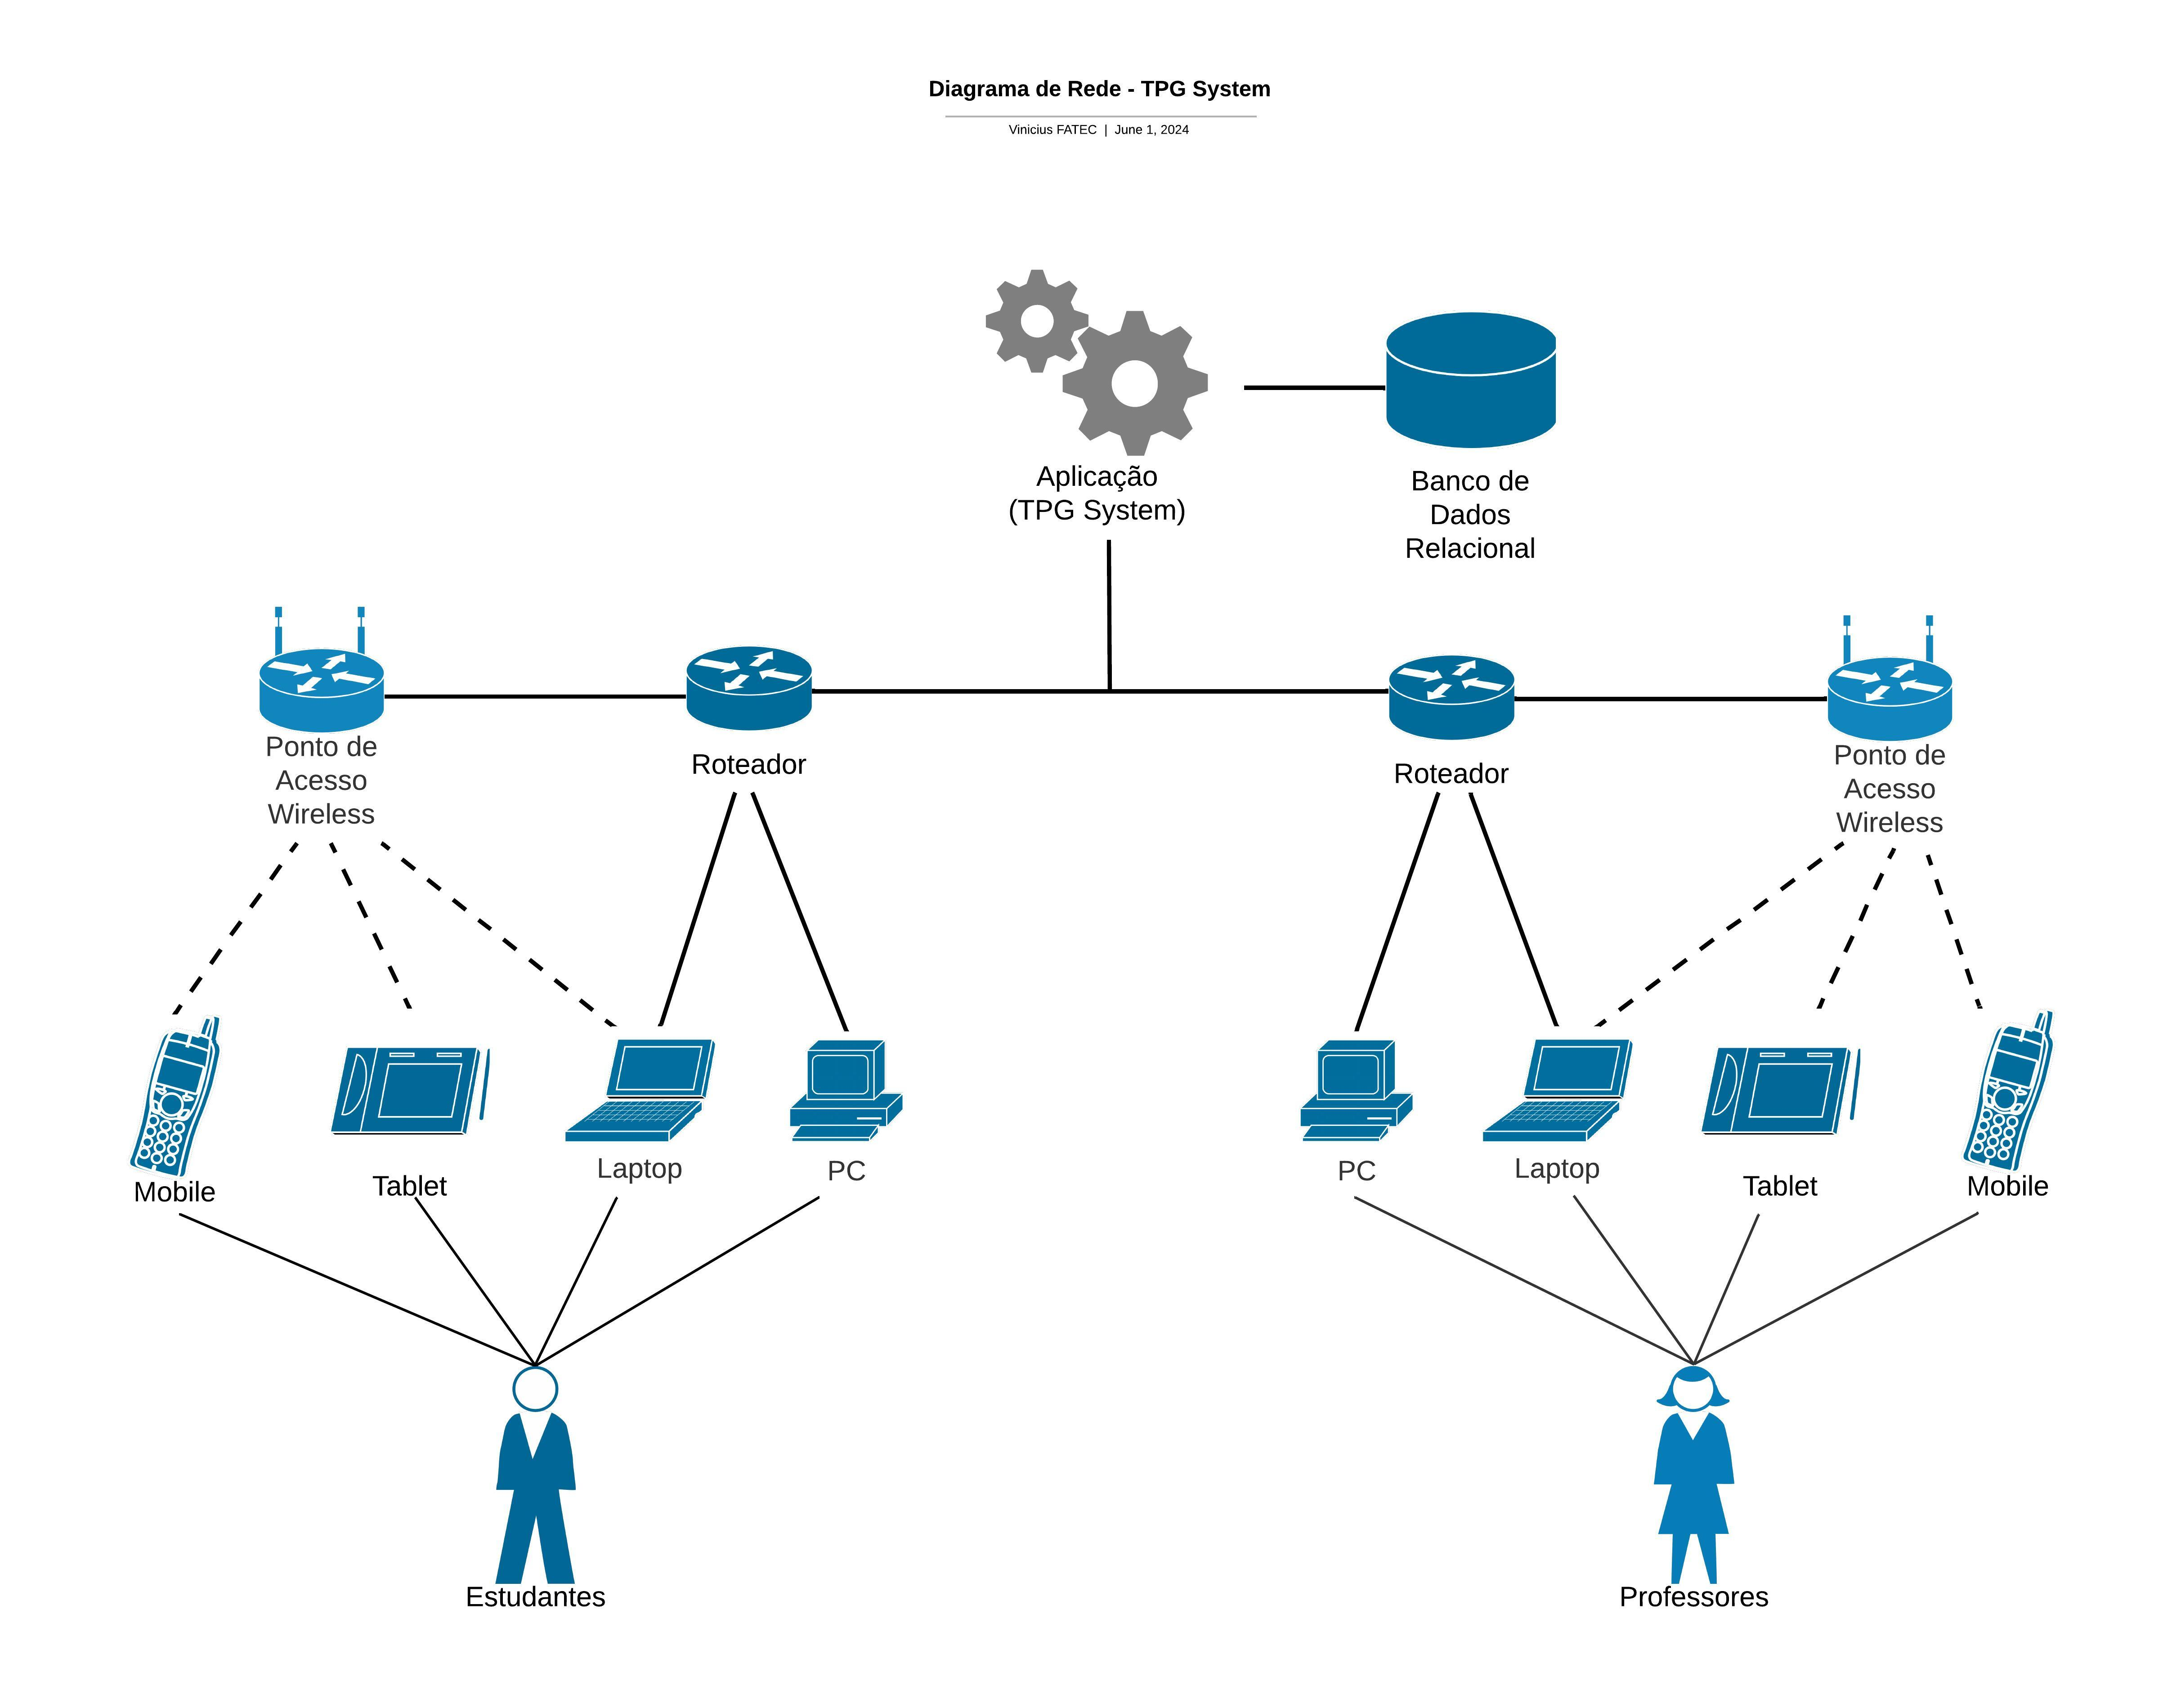
\includegraphics[scale=0.32]{Illustrations/dgR.jpg}
\SourceOrNote{Autoria Própria (2024)}
\end{flowchart}

\\
\begin{enumerate}
\item \textbf{Visualização das Atividades e Dependências:} Ajuda a visualizar todas as tarefas necessárias para a conclusão do projeto, bem como suas interdependências. Isso facilita a compreensão de como as atividades se relacionam e se influenciam mutuamente;  
\\ 
\item \textbf{Planejamento e Sequenciamento: } Permite identificar a sequência lógica das atividades, o que é crucial para o planejamento eficiente do cronograma do projeto;
\\
\item \textbf{Identificação do Caminho Crítico:} O diagrama ajuda a identificar o caminho crítico, ou seja, a sequência de atividades que determina a duração total do projeto. Isso é vital para gerenciar prazos e garantir que o projeto seja concluído no tempo estimado; 
\\
\item \textbf{Gestão de Recursos:} Facilita a alocação e o gerenciamento de recursos, identificando onde e quando recursos específicos serão necessários;  
\\ 
\item \textbf{Análise de Riscos e Problemas:} Permite uma análise mais detalhada de possíveis riscos e gargalos no projeto, ajudando a antecipar e mitigar problemas antes que eles ocorram;
\\
\item \textbf{Comunicação e Colaboração:} Serve como uma ferramenta de comunicação eficiente entre membros da equipe e partes interessadas, promovendo uma melhor colaboração e entendimento compartilhado do progresso do projeto; 
\\
\end{enumerate}

\begin{itemize}

\item \textbf{Análise de implementação de algoritmos de ordenação e sua eficácia na aplicação:}
\\

\end{itemize}

Ao considerar várias situações hipotéticas, a mais crítica é o desenvolvimento de um relatório pedagógico que mostre a realidade cotidiana. Com base nesse apontamento, pensou-se no seguinte cenário:
\\

Uma unidade escolar com 7 salas de aula, sendo uma de cada ano/série (6º ano, 7º ano, 8º ano, 9º ano, 1ª série EM, 2ª série EM, 3ª série EM), contendo em média 40 estudantes regularmente matriculados e frequentes. Cada sala de aula possui em média 12 professores, correspondendo a 12 componentes curriculares. Um componente curricular possui em média 30 habilidades. Um professor necessita retirar um relatório pedagógico, em ordem decrescente, contendo todos os estudantes que mais desenvolveram habilidades (\Cref{fig:MergeSort.jpg}).
\\
\begin{figure}[!h]
\centering
\caption{Algorítimo de Ordenação: MergeSort - TPG System}%
\label{fig:MergeSort.jpg}
\includegraphics[scale=0.42]{Illustrations/MergeSort.jpg}
\SourceOrNote{Autoria Própria (2024)}
\end{figure}

O algoritmo de ordenação Merge Sort apresenta um desempenho consistente e garante uma complexidade de tempo de O(n log n), além de manter a estabilidade, preservando a ordem relativa dos elementos iguais. Embora exija espaço adicional de memória para criar arrays auxiliares durante a mesclagem, sua vantagem reside na facilidade de implementação em comparação com o QuickSort. Para este teste, que não envolve uma quantidade moderada de dados e não foram mencionadas preocupações com estabilidade ou restrições de memória, o QuickSort poderia ser uma escolha razoável. Este método normalmente oferece um desempenho rápido e é amplamente empregado em diversos cenários. No entanto, por trabalharmos em um ambiente real com grande fluxo de dados e a necessidade de estabilidade no processo, ou a garantia de desempenho no pior caso forem preocupações importantes, o MergeSort se torna a opção mais segura.



